% "{'classe':('PSI'),'chapitre':'chs_hs','type':('application'),'titre':'Exercices d\\'application', 'source':'Pôle Chateaubriand - Joliot-Curie','comp':('B2-16'),'corrige':False}"
%\setchapterimage{bandeau}
\chapter*{Application \arabic{cptApplication} :\\ 
Exercices d'application -- \ifprof Corrigé \else Sujet \fi}
\addcontentsline{toc}{section}{Application \arabic{cptApplication} : Exercices d'application -- \ifprof Corrigé \else Sujet \fi}

\iflivret \stepcounter{cptApplication} \else
\ifprof  \stepcounter{cptApplication} \else \fi
\fi

\setcounter{question}{0}
\marginnote{Pôle Chateaubriand -- Joliot-Curie.}
\marginnote{
\UPSTIcompetence[2]{B2-16}
}

%\begin{marginfigure}
%
%\end{marginfigure}


\subsection*{Exercice 1 --Applications directes}



\question{Pour chacun des mécanismes suivants, déterminer le degré d'hyperstatisme.}

\question{Lorsque le modèle est hyperstatique, proposer :}
\textit{
\begin{itemize}
\item des conditions d'assemblage (intuitivement);
\item un modèle isostatique.
\end{itemize}}
\begin{table*}[!h]
\begin{multicols}{3}
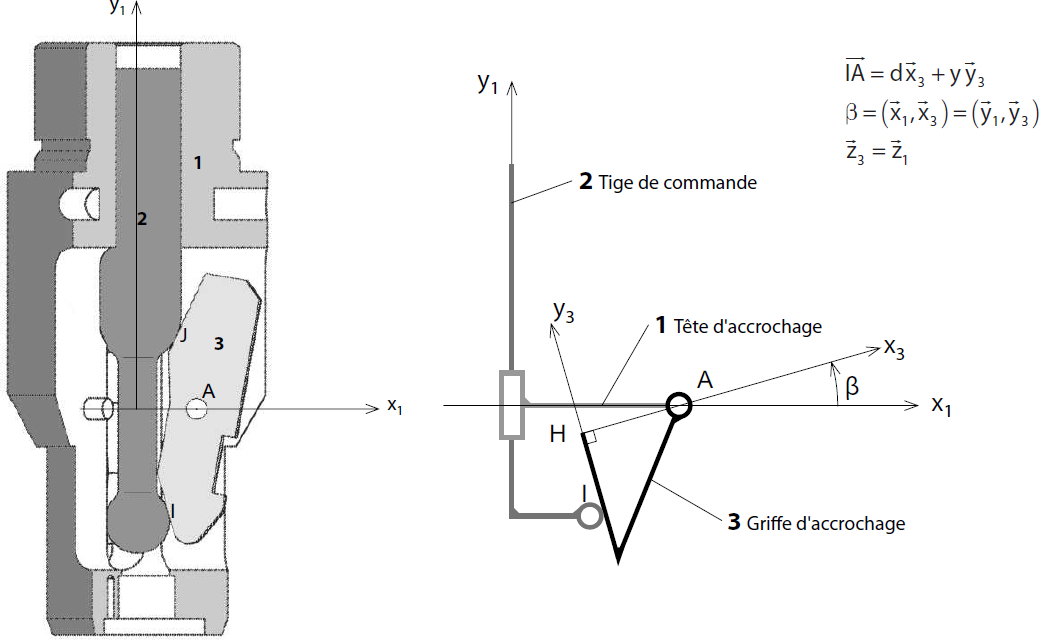
\includegraphics[width=.8\linewidth]{fig_01.png}
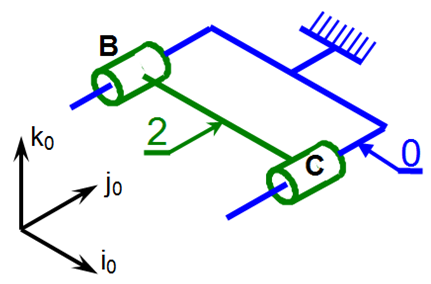
\includegraphics[width=.8\linewidth]{fig_02.png}
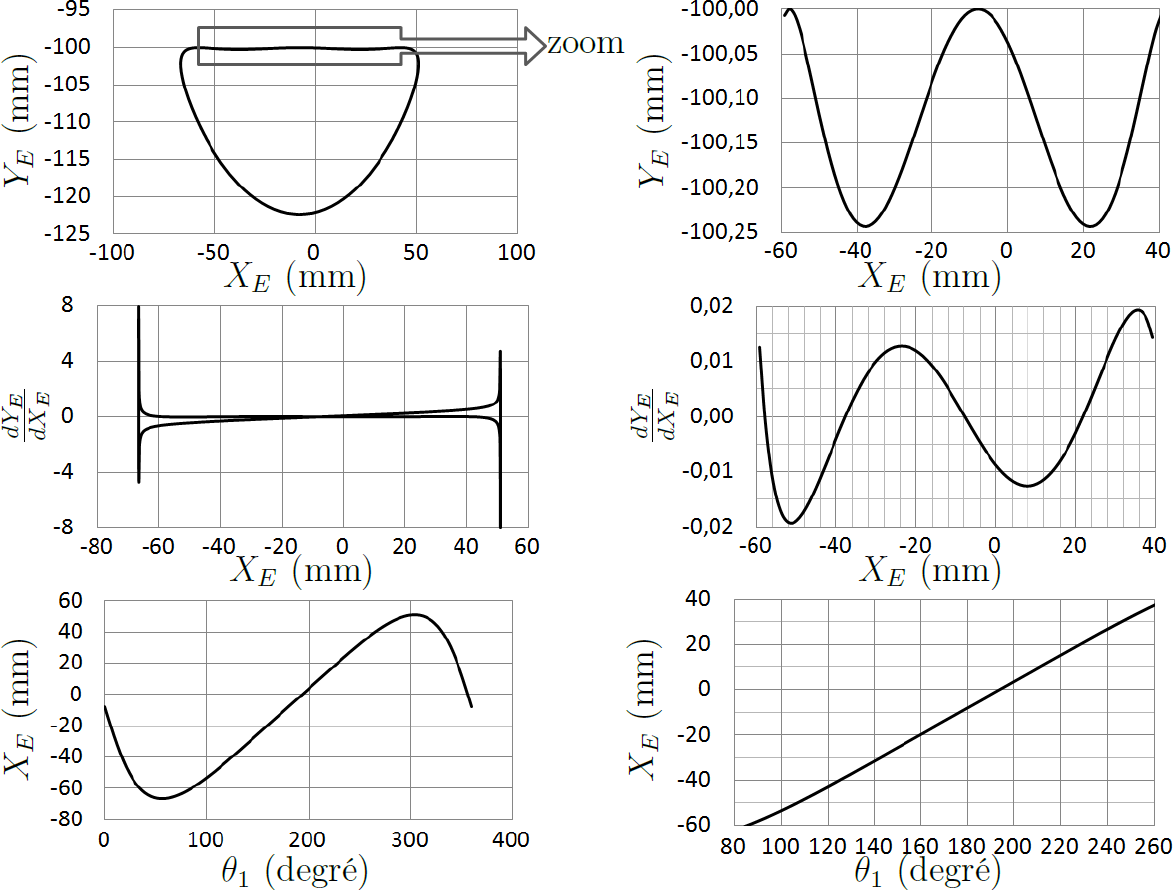
\includegraphics[width=.8\linewidth]{fig_03.png}
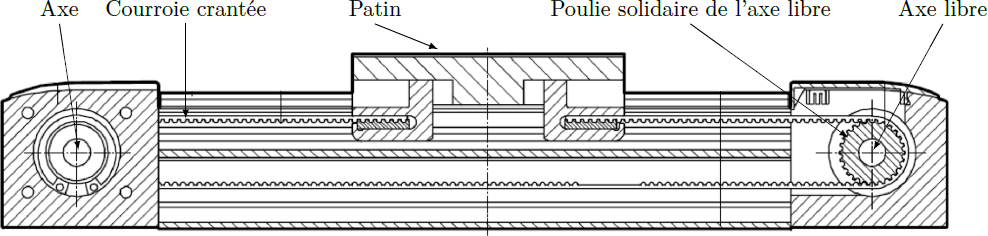
\includegraphics[width=.8\linewidth]{fig_04.png}
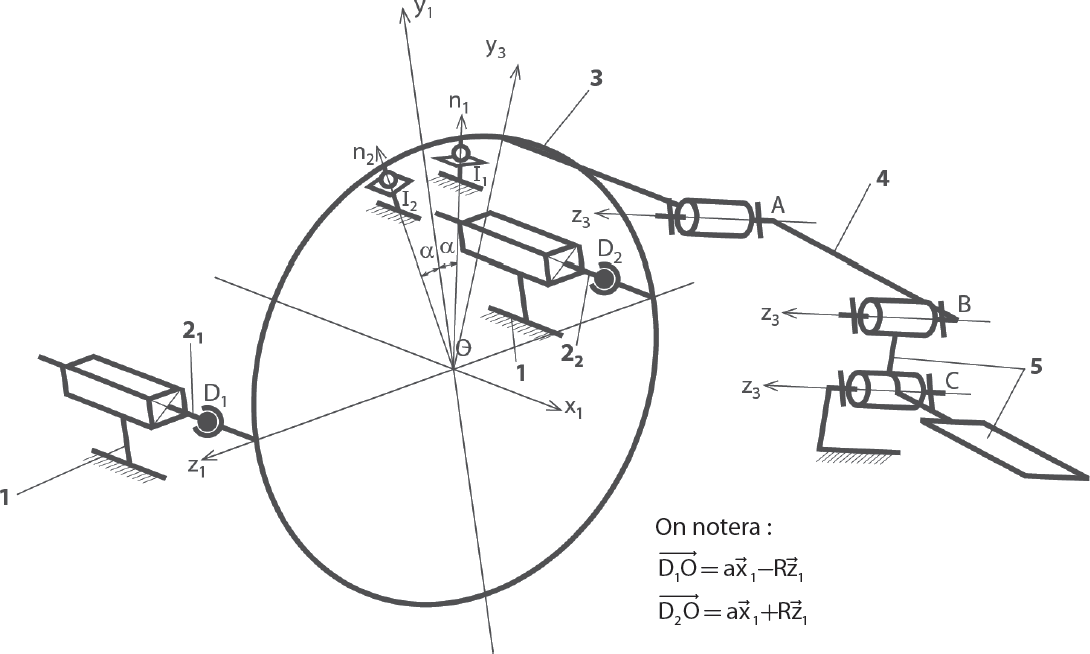
\includegraphics[width=.8\linewidth]{fig_05.png}
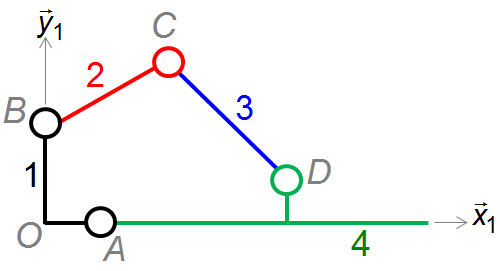
\includegraphics[width=.8\linewidth]{fig_07.png}
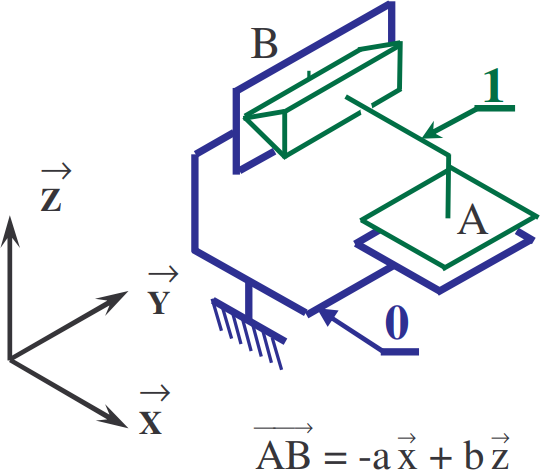
\includegraphics[width=.8\linewidth]{fig_08.png}
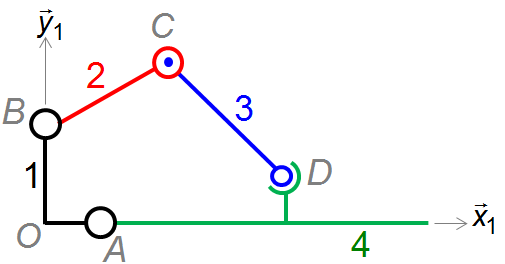
\includegraphics[width=.8\linewidth]{fig_09.png}
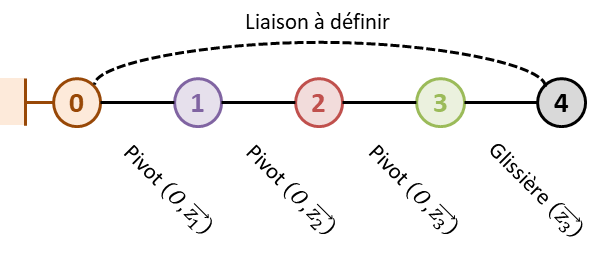
\includegraphics[width=.8\linewidth]{fig_10.png}
\end{multicols}
\end{table*}

\newpage

\subsection*{Exercice 2 -- Déphasage d'arbre à cames}

\marginnote{Banque PT SIA -- 2008.}


L'optimisation d'un moteur 4 temps passe (entre autre) par une bonne maîtrise des lois de levée des soupapes. Il est ainsi possible de positionner entre la poulie \textbf{1} (entraînée par le vilebrequin via une chaîne) et l'arbre à came  \textbf{2} un système permettant de créer un déphasage entre ces pièces. 

\begin{marginfigure}
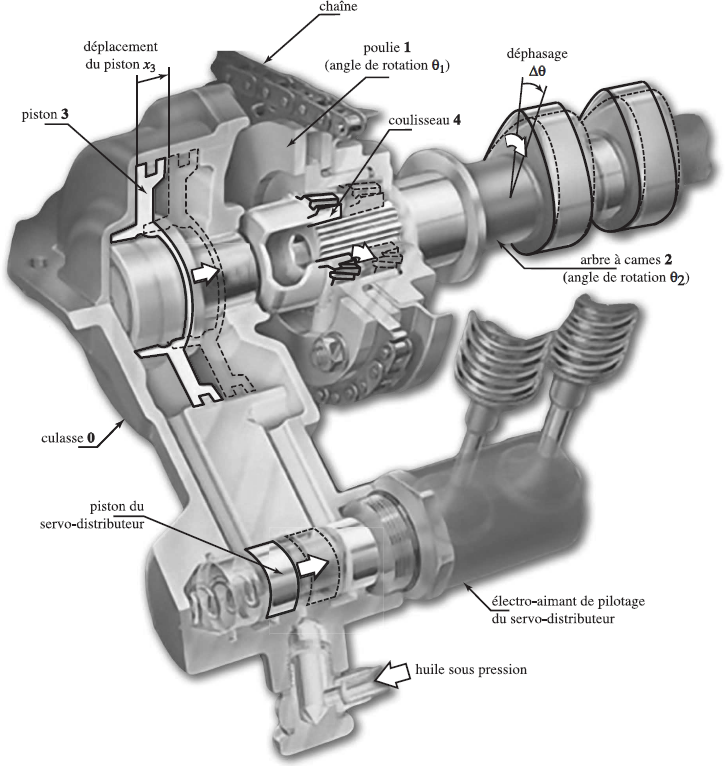
\includegraphics[width=\linewidth]{calage_1.png}
\end{marginfigure}

On propose ci-dessous un modèle cinématique du système de déphasage. On retrouve la culasse \textbf{0}, la poulie d’entraînement \textbf{1}, l'arbre à cames \textbf{2}, le piston \textbf{3} et le coulisseau \textbf{4}. 


\begin{center}
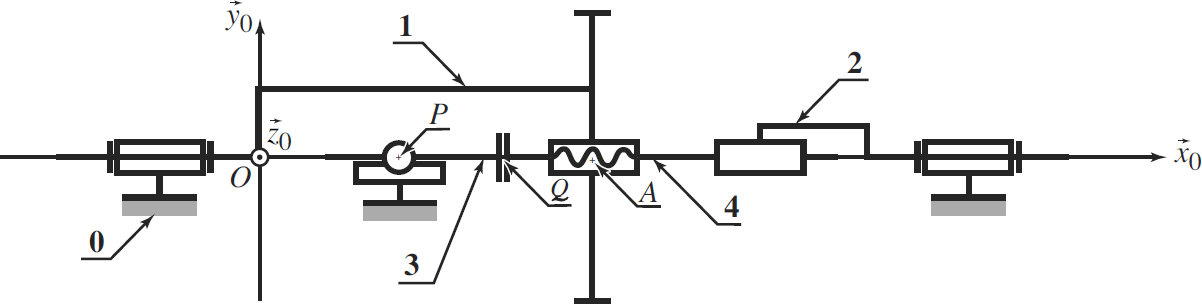
\includegraphics[width=.8\linewidth]{calage_2.png}
\end{center}

\question{Établir le graphe des liaisons du mécanisme.}
\ifprof
\begin{corrige}
\end{corrige}\else\fi

\question{Déterminer le degré d'hyperstatisme en précisant la démarche utilisée. (On utilisera la méthode cinématique et la méthode statique).}
\ifprof
\begin{corrige}
\end{corrige}\else\fi

\subsection*{Exercice 3 -- Simulateur de vol pour la formation de pilotes en aéroclub}


\begin{flushright}
\textit{Centrale Supelec 2017 -- PSI.}
\end{flushright}
On s’intéresse à un simulateur de vol à plate-forme dynamique. 
%
%\begin{center}
%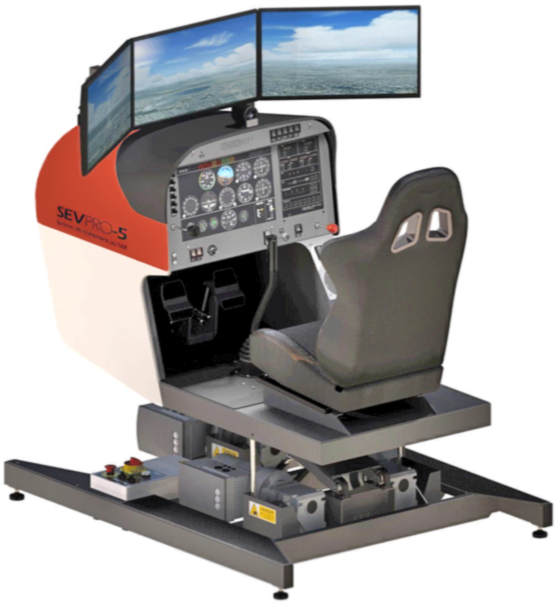
\includegraphics[width=.7\linewidth]{aero_01.png}
%\end{center}
Deux moteurs permettent d'assurer le mouvement de tangage.  Ils entraînent respectivement les liaisons pivots de centres $H$ et $O$. 

\begin{marginfigure}
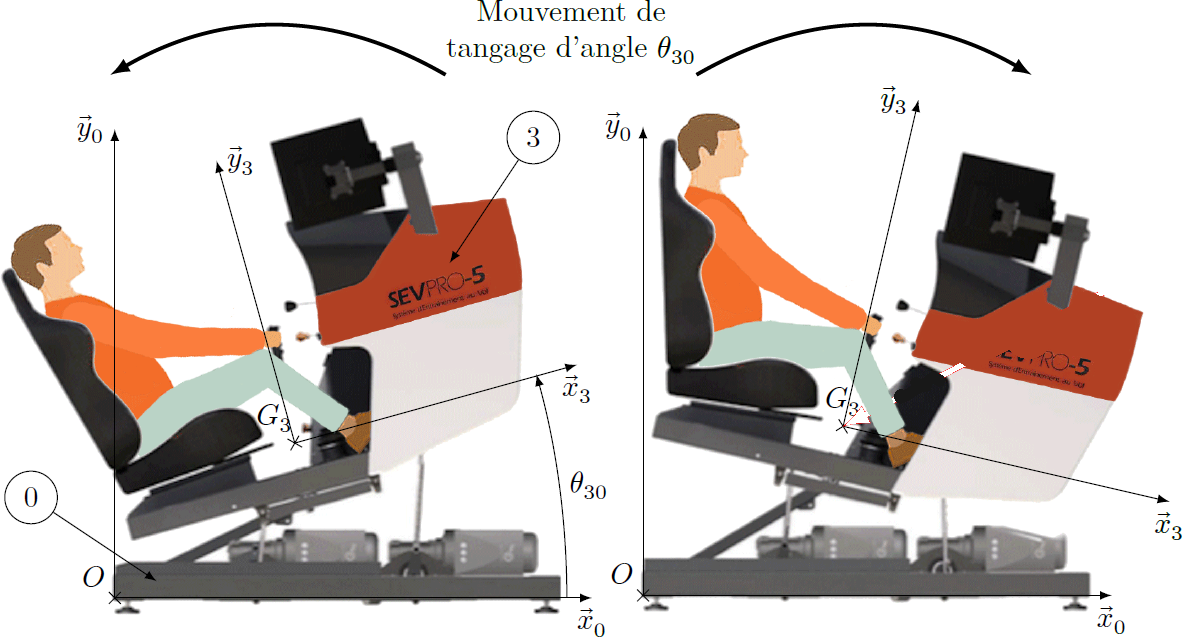
\includegraphics[width=\linewidth]{aero_04.png}
\end{marginfigure}

On propose le modèle plan suivant (la pièce 6 est en traits pointillés pour la démarquer des autres pièces).

\question{Déterminer le degré d'hyperstatisme du modèle proposé.}

\begin{center}
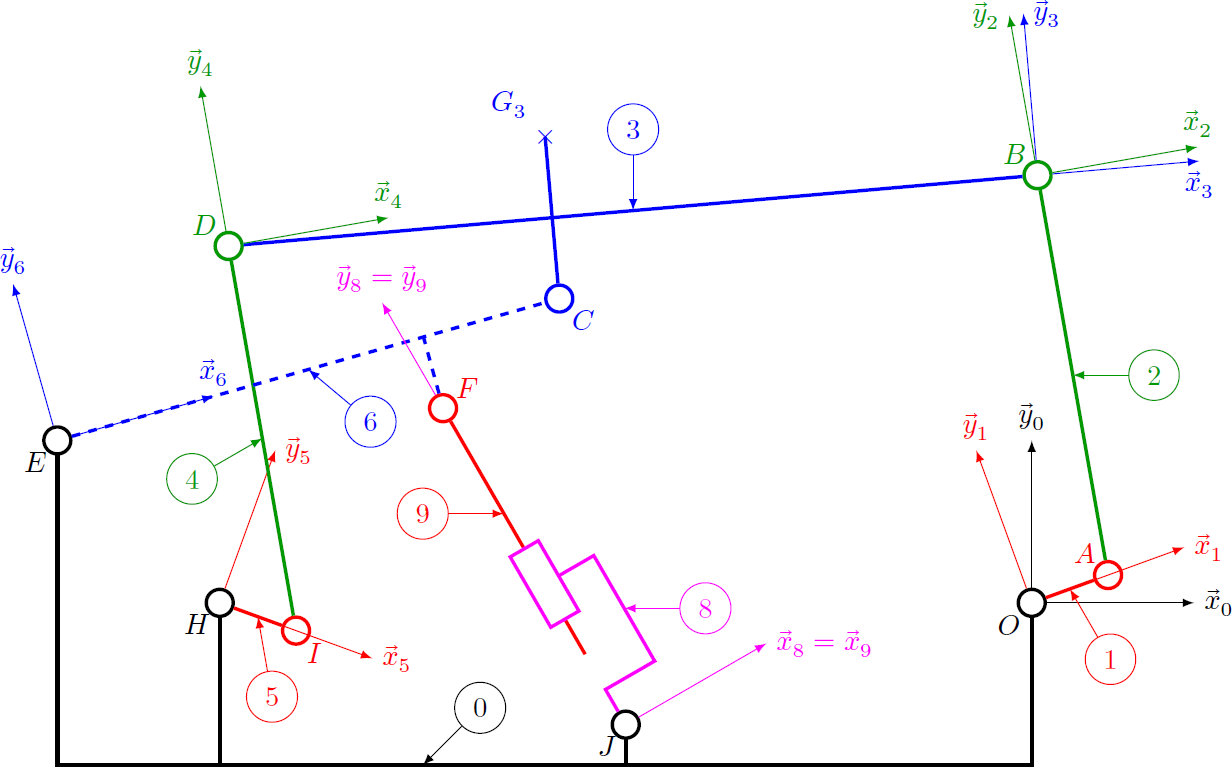
\includegraphics[width=.8\linewidth]{aero_06.png}
\end{center}

%\subsection*{Exercice 4 -- Chariot élévateur de bateaux}
%On donne le schéma cinémétique et le graphe de liaisons associés au chariot élévateur de bateaux. 
%\setcounter{exo}{0}
%\question{Déterminer le degré d'hyperstatisme du modèle.}
%\begin{center}
%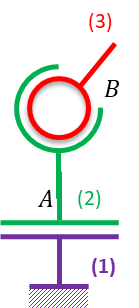
\includegraphics[width=.8\linewidth]{fig_11.png}
%%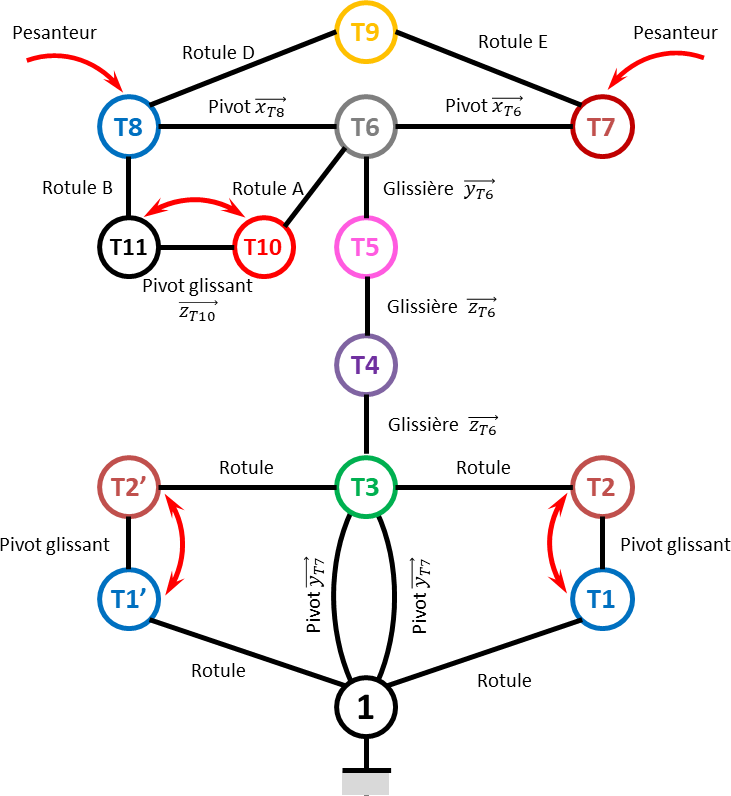
\includegraphics[width=.45\linewidth]{fig_12.png}
%\end{center}
%
%\begin{center}
%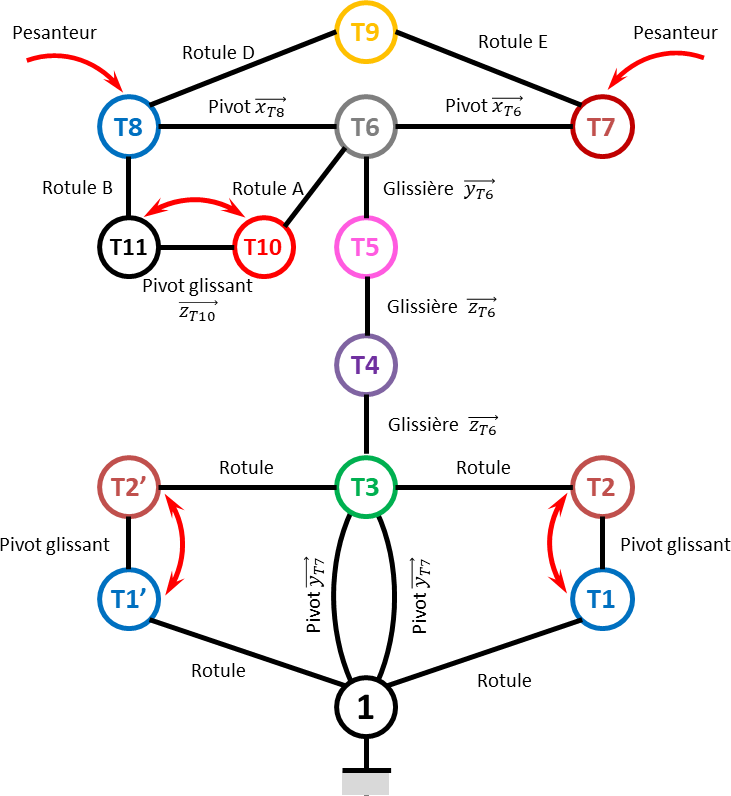
\includegraphics[width=.8\linewidth]{fig_12.png}
%%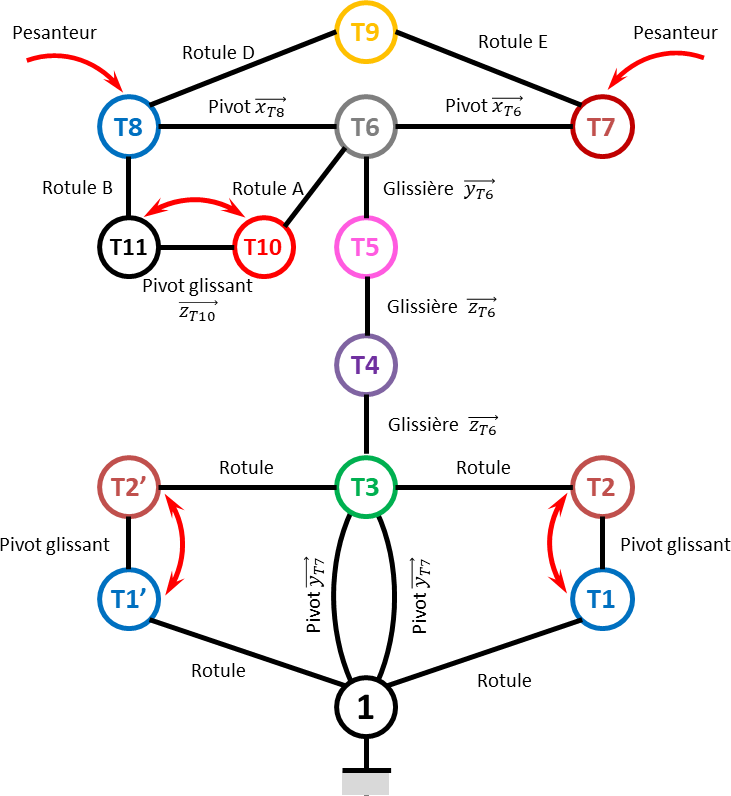
\includegraphics[width=.45\linewidth]{fig_12.png}
%\end{center}
%
%
%%\vspace{3cm}
%%
%%\subsection*{Éléments de corrigé}
%


\subsection*{Exercice 5 -- Pousseur de tablier}

\marginnote{Banque PT 2008 -- SIC.}



Une technique pour construire un pont et de commencer par ériger les piles définitives en béton et les piles
temporaires en acier. On peut alors assembler tronçon par tronçon, les 2 tabliers sur la terre ferme et enfin
pousser les deux parties du tablier assemblées sur les piles afin de réaliser la jonction.
Cette opération de poussée est réalisée à l’aide de systèmes hydrauliques nommés « pousseurs
de tablier ». 
\begin{marginfigure}
\centering
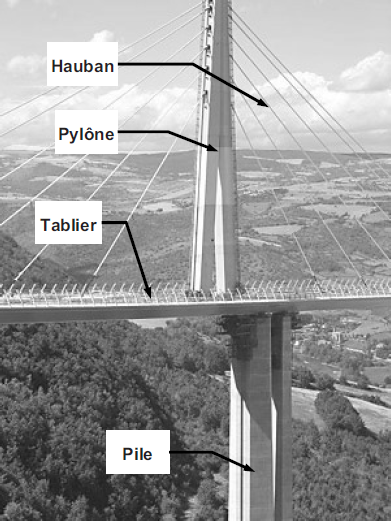
\includegraphics[width=.6\linewidth]{viaduc_01.png}
\end{marginfigure}

Le pousseur de tablier est soutenu par plusieurs vérins de balancelle verticaux (non étudiés) qui assurent le positionnement de la semelle afin que la cale de poussée soit parallèle et à la bonne distance du plan inférieur du tablier. 

\begin{marginfigure}
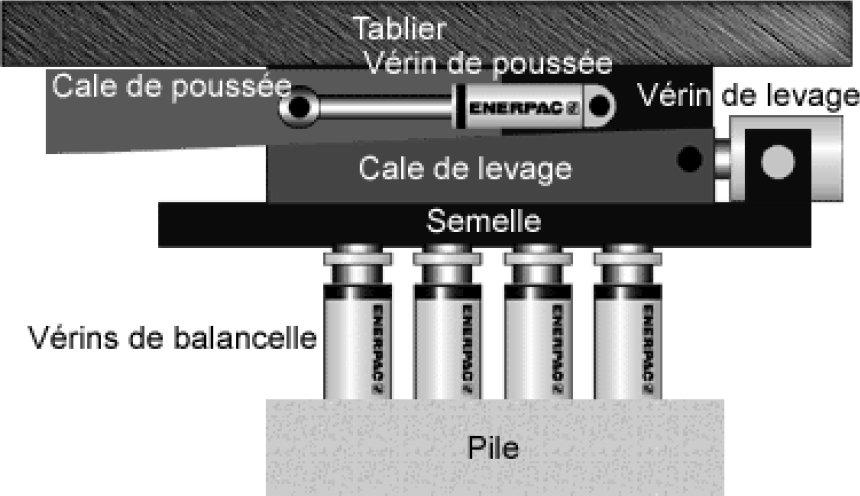
\includegraphics[width=\linewidth]{viaduc_02.png}
\end{marginfigure}


On suppose dans cette partie, que l’angle que fait le plan supérieur de la cale de levage avec
l’horizontale est petit. Ce qui revient à considérer que les contacts dans les liaisons planes sont
maintenus durant tout le mouvement.
Une première étude conduit à la modélisation suivante.

\begin{marginfigure}
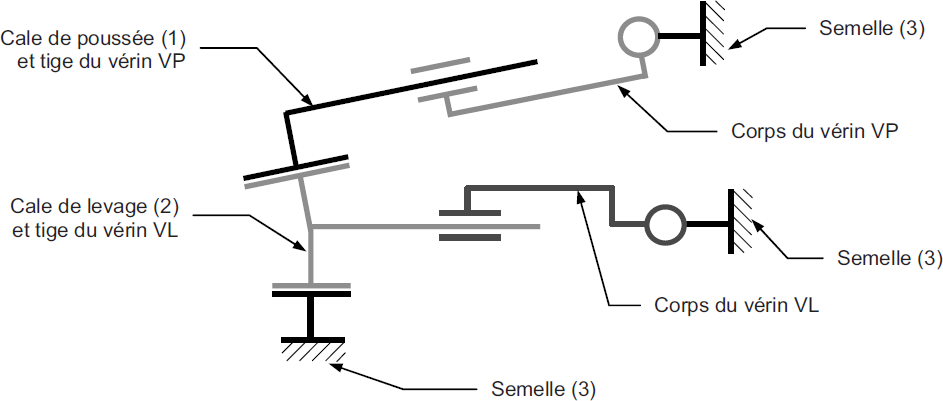
\includegraphics[width=\linewidth]{viaduc_03.png}
\end{marginfigure}

\question{Proposer un modèle pour tenir compte de l'hypothèse des angles <<~petits~>>.}
\ifprof
\begin{corrige}
\end{corrige}\else\fi

\question{Estimer le degré de mobilité du modèle proposé.}
\ifprof
\begin{corrige}
\end{corrige}\else\fi


\question{Déterminer le degré d’hyperstatisme du modèle proposé.}
\ifprof
\begin{corrige}
\end{corrige}\else\fi


\question{Proposer des modifications pour rendre le système isostatique. Faire un
nouveau schéma cinématique tenant compte de ces modifications.}
\ifprof
\begin{corrige}
\end{corrige}\else\fi



\begin{marginfigure}
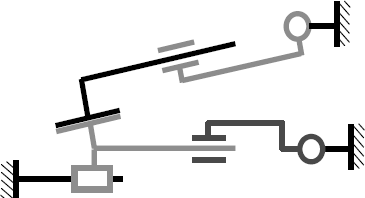
\includegraphics[width=.8\linewidth]{viaduc_04.png}
\end{marginfigure}


\question{Le constructeur a fait le choix de mettre
une liaison glissière de direction horizontale à la place de
la liaison plane entre la cale de levage (2) et la semelle (3)
(figure 6). Qu’est-ce qui justifie un tel choix ? Comment
peut-on rendre ce modèle isostatique ?}
\ifprof
\begin{corrige}
\end{corrige}\else\fi



\subsection*{Exercice 6 -- Planeur sous marin}

\marginnote{Banque PT 2012 -- SIC.}

\begin{marginfigure}
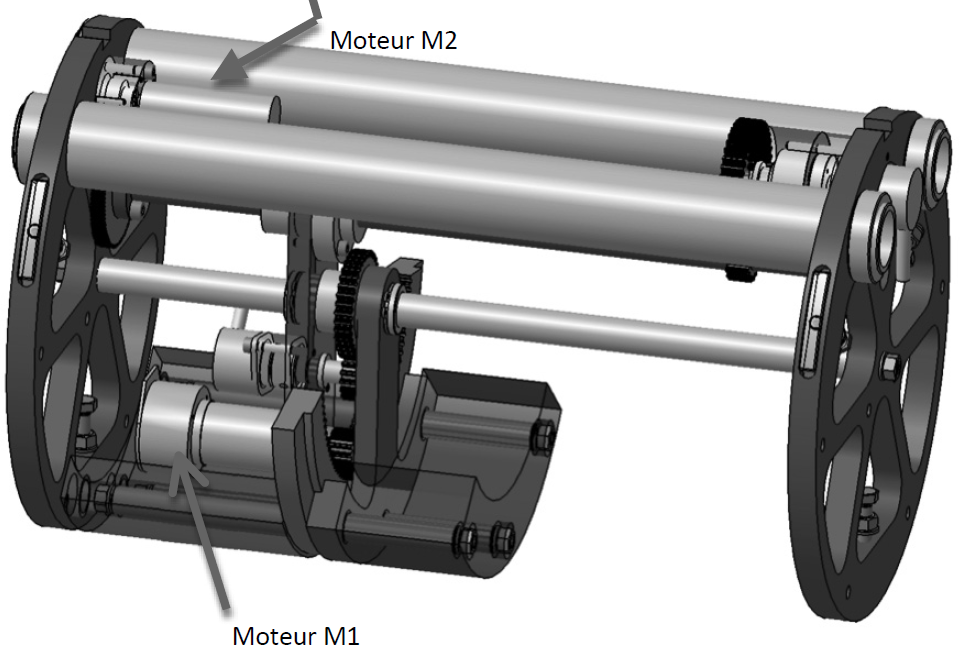
\includegraphics[width=.8\linewidth]{plan_01.png}
\end{marginfigure}

Le planeur sous-marin est un dispositif autonome développé par l'IFREMER dont le but est de réaliser des mesures océanographiques. Il ressemble à un mini sous-marin qui plane en dents de scie vers un point prédéfini. Il remonte régulièrement à la surface afin de communiquer avec son opérateur par satellite afin d'envoyer les données acquises pendant sa plongée pour évaluer sa dérive due aux courants. 


Dans le but de modifier l'orientation et l'équilibrage du planeur, l apartie centrale du planeur comporte un dispositif qui permet de positionner le centre de gravité axialement \textbf{24} et radialement \textbf{11}. 


\begin{center}
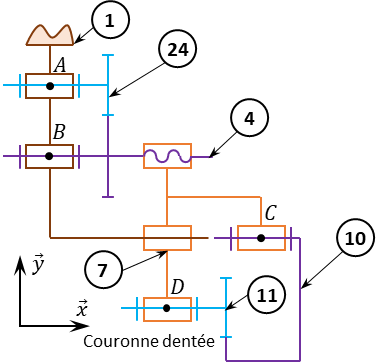
\includegraphics[width=.6\linewidth]{plan_02.png}
\end{center}


\question{Réaliser le graphe de liaison associé au schéma cinématique minimal proposé. Identifier le nombre de mobilités. }
\ifprof
\begin{corrige}
\end{corrige}\else\fi

On supposera que la liaison entre deux roues dentées est une liaison ponctuelle. 


\question{Déterminer le degré d'hyperstatisme. Si celui-ci est non nul, indiquer la ou les contraintes géométriques associées. }
\ifprof
\begin{corrige}
\end{corrige}\else\fi


